\documentclass[12pt]{amsart}
% packages
\usepackage{graphicx}
\usepackage{setspace}
\usepackage{amssymb,amsmath,amsthm,amsfonts,amscd}
\usepackage{hyperref}
\usepackage{color}
\usepackage{booktabs}
\usepackage{tabularx}
\usepackage{enumitem}
\usepackage[retainorgcmds]{IEEEtrantools}
\usepackage[notref,notcite,final]{showkeys}
\usepackage[final]{pdfpages}
\usepackage{fancyhdr}
\usepackage{upgreek}
\usepackage{multicol}

\usepackage{fancyvrb}
\usepackage{listings}
% set margin as 0.75in
\usepackage[margin=0.75in]{geometry}

% tikz-related settings
\usepackage{tikz}
\usepackage{tikz-cd}
\usetikzlibrary{cd}

% theorem environments with italic font
\newtheorem{thm}{Theorem}[section]
\newtheorem*{thm*}{Theorem}
\newtheorem{lemma}[thm]{Lemma}
\newtheorem{prop}[thm]{Proposition}
\newtheorem{claim}[thm]{Claim}
\newtheorem{corollary}[thm]{Corollary}
\newtheorem{conjecture}[thm]{Conjecture}
\newtheorem{question}[thm]{Question}
\newtheorem{procedure}[thm]{Procedure}
\newtheorem{assumption}[thm]{Assumption}

% theorem environments with roman font (use lower-case version in body
% of text, e.g., \begin{example} rather than \begin{Example})
\newtheorem{Definition}[thm]{Definition}
\newenvironment{definition}
{\begin{Definition}\rm}{\end{Definition}}
\newtheorem{Example}[thm]{Example}
\newenvironment{example}
{\begin{Example}\rm}{\end{Example}}

\theoremstyle{definition}
\newtheorem{remark}[thm]{\textbf{Remark}}

% special sets
\newcommand{\A}{\mathbb{A}}
\newcommand{\C}{\mathbb{C}}
\newcommand{\F}{\mathbb{F}}
\newcommand{\N}{\mathbb{N}}
\newcommand{\Q}{\mathbb{Q}}
\newcommand{\R}{\mathbb{R}}
\newcommand{\Z}{\mathbb{Z}}
\newcommand{\cals}{\mathcal{S}}
\newcommand{\ZZ}{\mathbb{Z}_{\ge 0}}
\newcommand{\cala}{\mathcal{A}}
\newcommand{\calb}{\mathcal{B}}
\newcommand{\cald}{\mathcal{D}}
\newcommand{\calh}{\mathcal{H}}
\newcommand{\call}{\mathcal{L}}
\newcommand{\calr}{\mathcal{R}}
\newcommand{\la}{\mathbf{a}}
\newcommand{\lgl}{\mathfrak{gl}}
\newcommand{\lsl}{\mathfrak{sl}}
\newcommand{\lieg}{\mathfrak{g}}

% math operators
\DeclareMathOperator{\kernel}{\mathrm{ker}}
\DeclareMathOperator{\image}{\mathrm{im}}
\DeclareMathOperator{\rad}{\mathrm{rad}}
\DeclareMathOperator{\id}{\mathrm{id}}
\DeclareMathOperator{\hum}{[\mathrm{Hum}]}
\DeclareMathOperator{\eh}{[\mathrm{EH}]}
\DeclareMathOperator{\lcm}{\mathrm{lcm}}
\DeclareMathOperator{\Aut}{\mathrm{Aut}}
\DeclareMathOperator{\Inn}{\mathrm{Inn}}
\DeclareMathOperator{\Out}{\mathrm{Out}}
\DeclareMathOperator{\Gal}{\mathrm{Gal}}


% frequently used shorthands
\newcommand{\ra}{\rightarrow}
\newcommand{\se}{\subseteq}
\newcommand{\ip}[1]{\langle#1\rangle}
\newcommand{\dual}{^*}
\newcommand{\inverse}{^{-1}}
\newcommand{\norm}[2]{\|#1\|_{#2}}
\newcommand{\abs}[1]{\lvert #1 \rvert}
\newcommand{\Abs}[1]{\bigg| #1 \bigg|}
\newcommand\bm[1]{\begin{bmatrix}#1\end{bmatrix}}
\newcommand{\op}{\text{op}}

% nicer looking empty set
\let\oldemptyset\emptyset
\let\emptyset\varnothing

\setlist[enumerate,1]{topsep=1em,leftmargin=1.8em, itemsep=0.5em, label=\textup{(}\arabic*\textup{)}}
\setlist[enumerate,2]{topsep=0.5em,leftmargin=3em, itemsep=0.3em}

%pagestyle
%\pagestyle{fancy} 

\begin{document}
\begin{center}
    \textsc{Random Walks. HW 2\\ Ian Jorquera\\ Collaboration: Tristan Neighbors}
\end{center}
\vspace{1em}


\definecolor{codegreen}{rgb}{0,0.6,0}
\definecolor{codegray}{rgb}{0.5,0.5,0.5}
\definecolor{codepurple}{rgb}{0.58,0,0.82}
\definecolor{backcolour}{rgb}{1,1,1}

\lstdefinestyle{mystyle}{
    backgroundcolor=\color{backcolour},   
    commentstyle=\color{codegray},
    keywordstyle=\color{magenta},
    numberstyle=\tiny\color{codegray},
    stringstyle=\color{codegreen},
    basicstyle=\ttfamily\footnotesize,
    breakatwhitespace=false,         
    breaklines=true,                 
    captionpos=b,                    
    keepspaces=true,                 
    numbers=left,                    
    numbersep=5pt,                  
    showspaces=false,                
    showstringspaces=false,
    showtabs=false,                  
    tabsize=2
}

\lstset{style=mystyle}


\begin{itemize}
\item[(1)] 
\begin{enumerate}[label=(\alph*)]
    \item There are $N_{n,a}$ total paths from $(0,0)$ to $(n,a)$. We can then use the reflection principal to determine the number of paths that go through or touch $-b$. To do this we will reflect over $-b$, That is we want to consider the number of paths that start at $(0,-2b)$ and go to $(n,a)$ these correspond to the paths that start at $(0,0)$ and touch $-b$, of which there are $N_{n,2b+a}$ of them. This means the number of paths that strictly stay above $-b$ and end at $a$ are $N_{n,a}-N_{n,2b+a}$.\\

    \item Now fix $n$ to be an even number. Notice that $P[X_1\geq 0, X_2\geq 0,\dots, X_{n-1}\geq 0]=P[X_1\geq 0, X_2\geq 0,\dots, X_{n-1}\geq 0, X_{n}\geq 0]$, because $X_{n-1}>0$ as $n-1$ is odd, meaning we know that $X_{n}\geq 0$. Furthermore because the step sizes are of size $1$ we know that any intermediate sum $X_i\geq 0$ is equivalent to $X_i>-1$. this allows us to sum over all possible positions for $X_n$ such that all previous positions were greater then $-1$, giving us

    \begin{align*}
        P[X_1\geq 0, X_2\geq 0,\dots, X_{n}\geq 0]=&P[X_1> -1, X_2>-1,\dots, X_{n}>-1]\\
        =&\sum_{r=0, r\text{ even}}^n P[X_1> -1, X_2>-1,\dots, X_{n-1}>-1, X_{n}= r]
    \end{align*}
    
    And from part (a) we know that 
    $$\sum_{r=0, r\text{ even}}^n P[X_1> -1, X_2>-1,\dots, X_{n-1}>-1, X_{n}= r]=\sum_{r=0,\\ r\text{ even}}^n \frac{N_{n,r}-N_{n,2+r}}{2^n}$$
    Which is a telescoping series such that the second term of the $r$ sum will cancel out the first term of the $r+2$ sum. So we are left with $\frac{N_{n,0}-N_{n,n+2}}{2^n}$, but $N_{n,n+2}=0$ so $P[X_1\geq 0, X_2\geq 0,\dots, X_{n}\geq 0]=\frac{N_{n,0}}{2^n}=P_n(0)$. And recall that $P[X_1> 0, X_2> 0,\dots, X_{n}> 0]=\frac{1}{2}P_n(0)$. Meaning $P[X_1> 0, X_2> 0,\dots, X_{n}> 0]=\frac{1}{2}P[X_1\geq 0, X_2\geq 0,\dots, X_{n-1}\geq 0]$.\\

    
\end{enumerate}

\item[(2)] My probability theory is very rusty so I referenced feller chapter 6 and this blog: \href{https://www.probabilitycourse.com/chapter11/11_1_2_basic_concepts_of_the_poisson_process.php}{here}.

\begin{enumerate}[label=(\alph*)]
% cant really do this. need to think about the prob of n people going to store then the prob of them buying book.
    \item If there are $20$ customers per hour and they buy a book with probability $1/5$ then we could model the number of people to enter a store with a Poisson distribution where $\lambda=20$ customers per hours. Now we know that the number of customers who enter the store in a time interval $\tau$ is a Poisson distribution with parameter $\lambda\tau=20\tau$. If $n$ customers enter the store there would then be probability of $(\frac{4}{5})^n$ that no books are sold. So we can sum over all the possible number of people to enter the store in the interval $\tau$, where no one buys a book. This would be
    
    \begin{align*}
        P\left[0 \text{ books are bought in the interval $\tau$}\right]&=
        \sum_{n=0}^\infty P(X=n)\cdot\left(\frac{4}{5}\right)^n\\
        &= \sum_{n=0}^\infty\frac{e^{-\lambda\tau}(\lambda\tau)^n}{n!}\cdot\left(\frac{4}{5}\right)^n\\
        &=e^{-\lambda\tau}\sum_{n=0}^\infty\frac{(\frac{4}{5}\lambda\tau)^n}{n!}\\
        &=e^{-\lambda\tau}e^{\frac{4}{5}\lambda\tau}=e^{-\frac{\lambda\tau}{5}}
    \end{align*}
    
    So over the interval of 1 hour(with $\lambda=20$) the probability of no customers buying books is $e^{-\frac{20\cdot 1}{5}}e^{-4}$.\\

    \item The probability that no customers buy a book in the time interval $\tau$ is $e^{-4\tau}$. Which means that the probability that the first time a book is bought is in the time interval $\tau$ is $1-e^{-4\tau}$. Let $p(\tau)$ be the probability density function of the time until the first book is sold. We want want to following to be true 
    $$\int_{0}^{\tau}p(t)dt=1-e^{-\lambda\tau}$$
    Using the fundamental theorem of calculus we can then determine that the probability density function is $$p(\tau)=\frac{d}{d\tau}\left[\int_{0}^{\tau}p(t)dt\right]=\frac{d}{d\tau}\left[1-e^{-\lambda\tau}\right]=\lambda e^{-\lambda\tau}$$ So the probability density function is $p(\tau)=4e^{-4\tau}$.\\

    \item[(3)]
    \begin{enumerate}[label=(\alph*)]
        \item Let the following function define the probability of a step in a random walk whose steps are i.i.d.
    $$
p(x)=
    \begin{cases}
        p & \text{if } x=1\\
        1-p & \text{if } x=-1\\
        0 & \text{otherwise} 
    \end{cases}$$
In this case we can determine that the characteristic function is $\lambda(\theta)=\ip{e^{i\theta x}}=pe^{i\theta}+(1-p)e^{-i\theta}$. We can then use this with the binomial theorem to determine that 
$$\lambda^n(\theta)=\left(pe^{i\theta}+(1-p)e^{-i\theta}\right)^n=\sum_{k=0}^n {n \choose k} (pe^{i\theta})^{n-k}((1-p)e^{-i\theta})^k$$
Which means for $n=8$ steps, we would look at the coefficient of the constant term, which is when $k=4$. This gives us a probability of ${8\choose 4}p^4(1-p)^4$ and for $p=.6$ we have that $P[X_8=0]=0.2322$.\\

\item To maximize this probability we can find that $\frac{d}{dp}\left[p^4(1-p)^4\right]=4p^3\left(1-p\right)^4-4p^4\left(1-p\right)^3=0$ when $p=.5$, and graphically or when any concavity rules we can determine that this maximizes the probability $P[X_8=0]$. I'm skipping over my work here but this can be determined fairly easily using a graph(shown below).

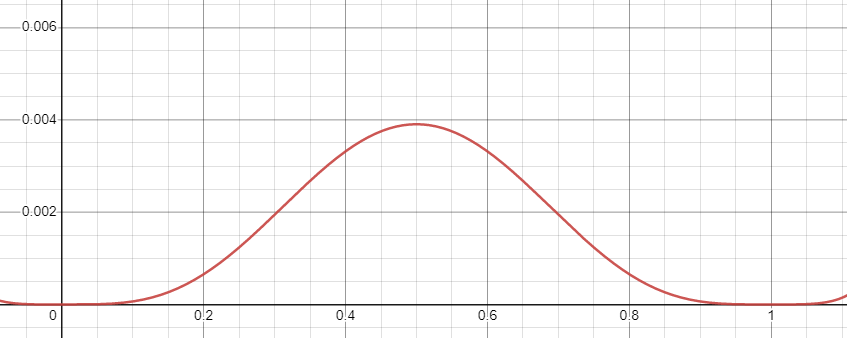
\includegraphics[scale=.5]{maximum_thing.png}
\\
% make this better

\item Let $p=.5$ and $n=40$. Recall the in a path of length $2n(=40)$ such that $2k$ was the last time at the origin we have that 

\begin{align*}
    \alpha_{2k,2n}&=P[X_{2k}=0,X_{2k+1}\neq 0,X_{2k+2}\neq 0,\dots,X_{2n}\neq 0]\\
    &=P[X_{2k+1}\neq 0,X_{2k+2}\neq 0,\dots,X_{2n}\neq 0|X_{2k}=0]\cdot P[X_{2k}=0]
\end{align*}

 by Bayes Theorem. Furthermore we know that $P[X_{2k}=0]=P_{2k}(0)$ and by the ballot theorem that 
 \begin{align*}
     P[X_{2k+1}\neq 0,X_{2k+2}\neq 0,\dots,X_{2n}\neq 0|X_{2k}=0]&=P[X_1\neq 0,X_{2}\neq 0,\dots,X_{2n-2k}\neq 0]\\
     &=P_{2n-2k}(0)
 \end{align*}
 
 Meaning $\alpha_{2k,2n}=P_{2n-2k}(0)P_{2k}(0)$. Recall that $P_n(0)=\frac{1}{2^n}{n \choose \frac{n}{2}}$, because to return to zero there must be an equal number of $+1$ and $-1$. This gives us the probability mass function 
$$p(k)=\alpha_{k,40}=
    \begin{cases}
        \alpha_{k,40} & \text{if } k \text{ is even}\\
        0 & \text{otherwise} 
    \end{cases}=\frac{1}{2^{40}}{40-k \choose \frac{40-k}{2}}{k \choose \frac{k}{2}}$$
    Notice that this function is zero when $k$ is odd. We can plot this function along side the arcsine distribution to see that 
    
    \begin{center}
    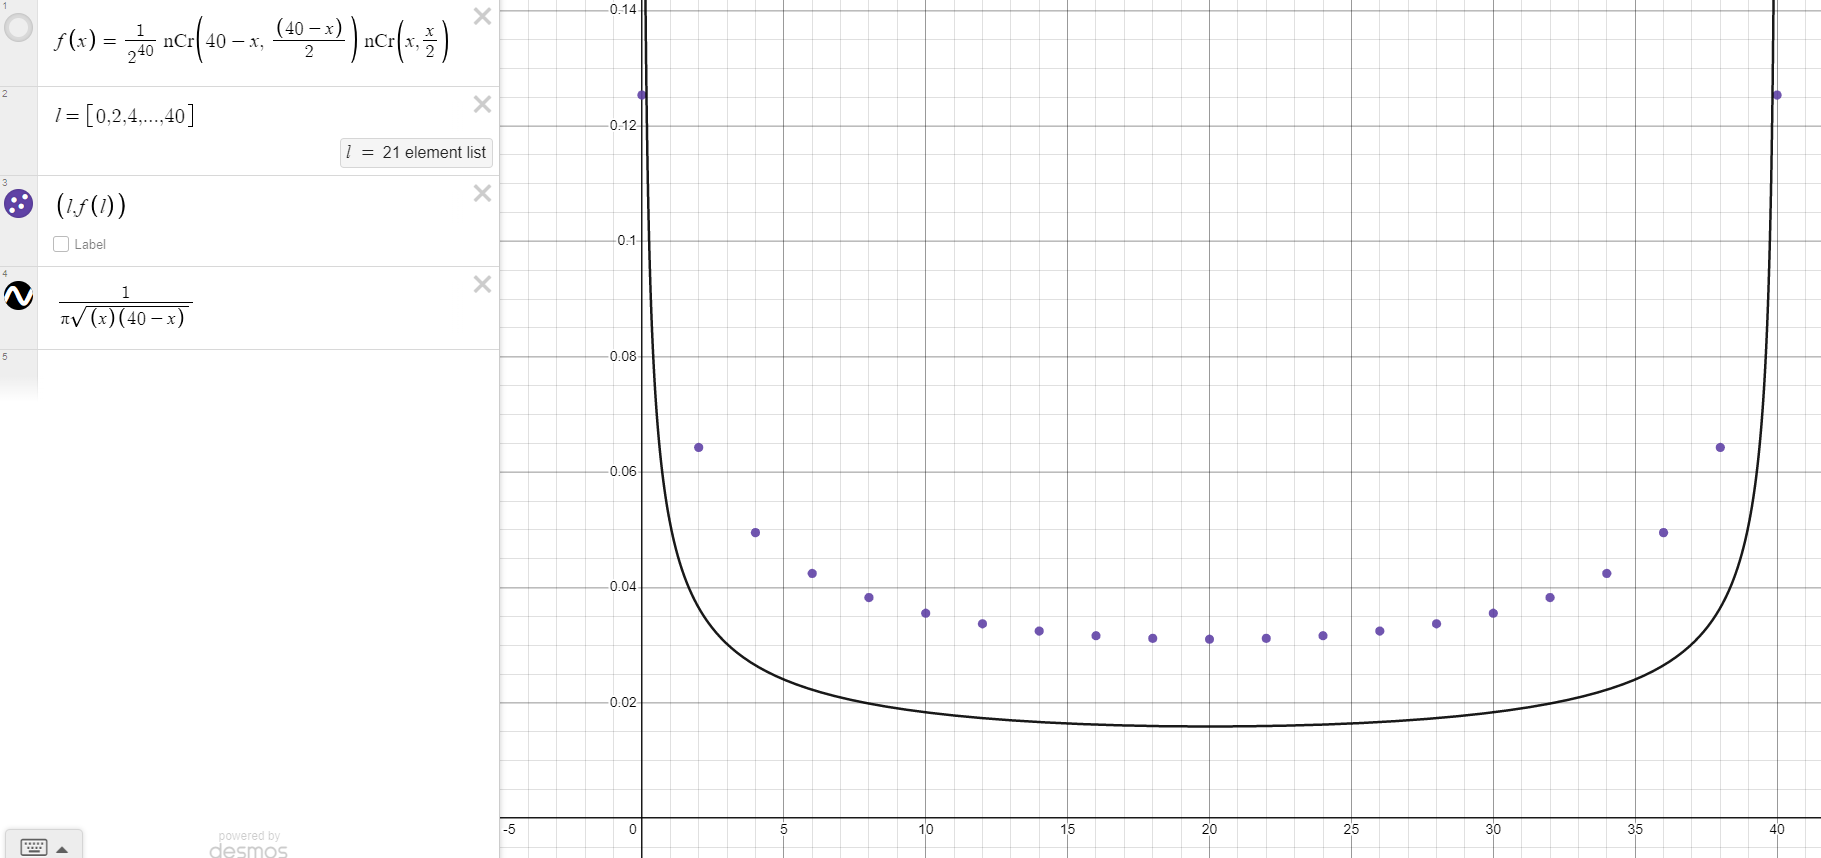
\includegraphics[scale=.3]{rw-p3-pmf.png}
    \end{center}

\end{enumerate}
\newpage
\item[(4)] 
\begin{enumerate}[label=(\alph*)]
    \item First we will plot the displacement of the Guassian random walk
    
    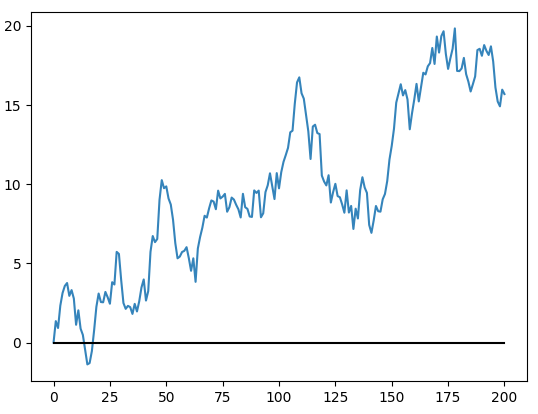
\includegraphics[scale=.5]{rw-hw2-gaussian.png}

    And then the displacement of the Cauchy random walk

    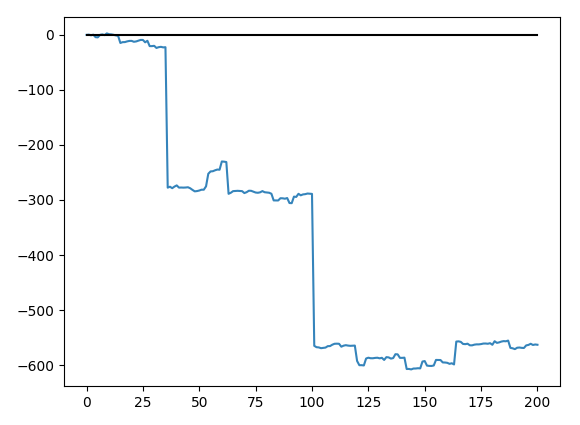
\includegraphics[scale=.5]{rw-hw2-cauchy.png}

    \item
    Now we will look at the sample mean(shown in blue) and the sample second moment(shown in orange) for the Gaussian

    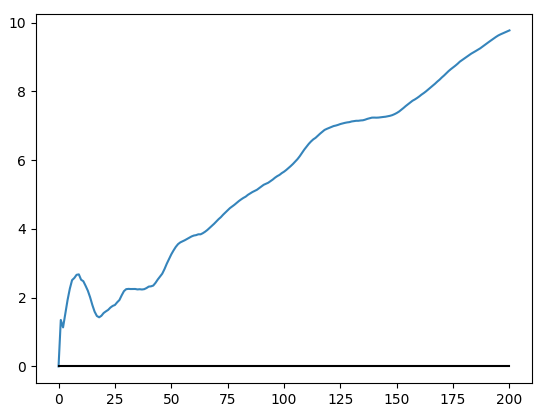
\includegraphics[scale=.5]{rw-hw2-gaussian-xbar.png}
    
    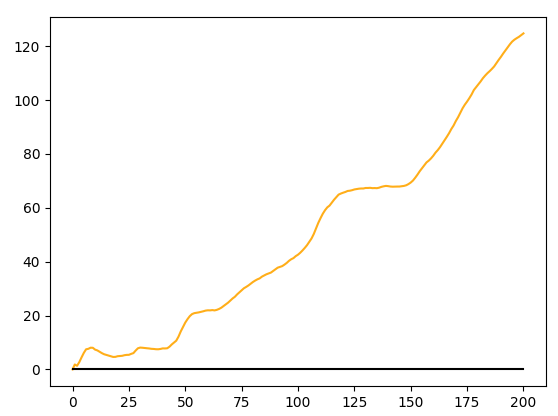
\includegraphics[scale=.5]{rw-hw2-gaussian-x2bar.png}

    Its difficult to tell but it is very possible the second moment is following a $n^2$ pattern. And then the same for the Cauchy random walk

    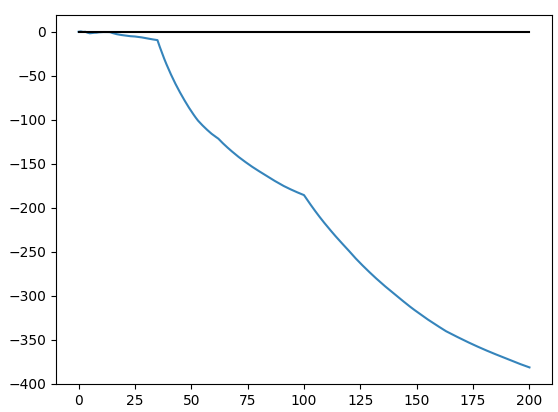
\includegraphics[scale=.5]{rw-hw2-cauchy-xbar.png}
    
    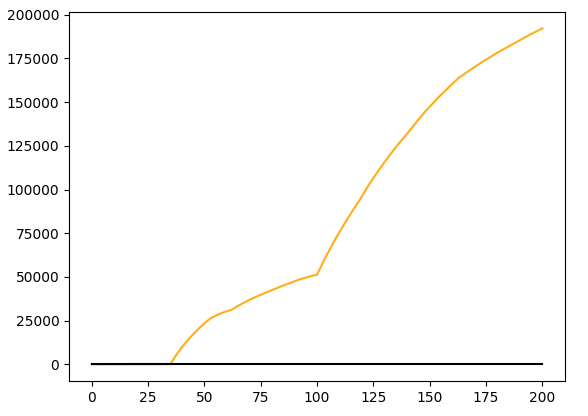
\includegraphics[scale=.5]{rw-hw2-cauchy-x2bar.png}

    In this case the second moment appears to be diverging

    \item From the central limit theorem we know that for large $x$, the displacement of the random walk from (A) with Gaussian distributed steps will have a probability density function being Gaussian with variance $n$. This means the second moment $\ip{x^2}=n^2$.\\% might want to show this
\end{enumerate}
\newpage
\item[(5)] To show the ballot theorem numerically I have created a Monte Carlo like simulation that generates $50000$ random walks from $(0,0)$ to $(p+q,p-q)$ and counts the number of walks that stay above zero. The code is provided below. I then tested this for $p+q=100$ and varied $p$ between $51$ and $100$.\\

I compared the probabilities found using this simulation with the expected probability of $\frac{p-q}{p+q}$ and got the follow plot for probability vs $p$. Where the orange represents $\frac{p-q}{p+q}$ and the blue represents the simulated probability. We can see that they seem to match with a high correlations

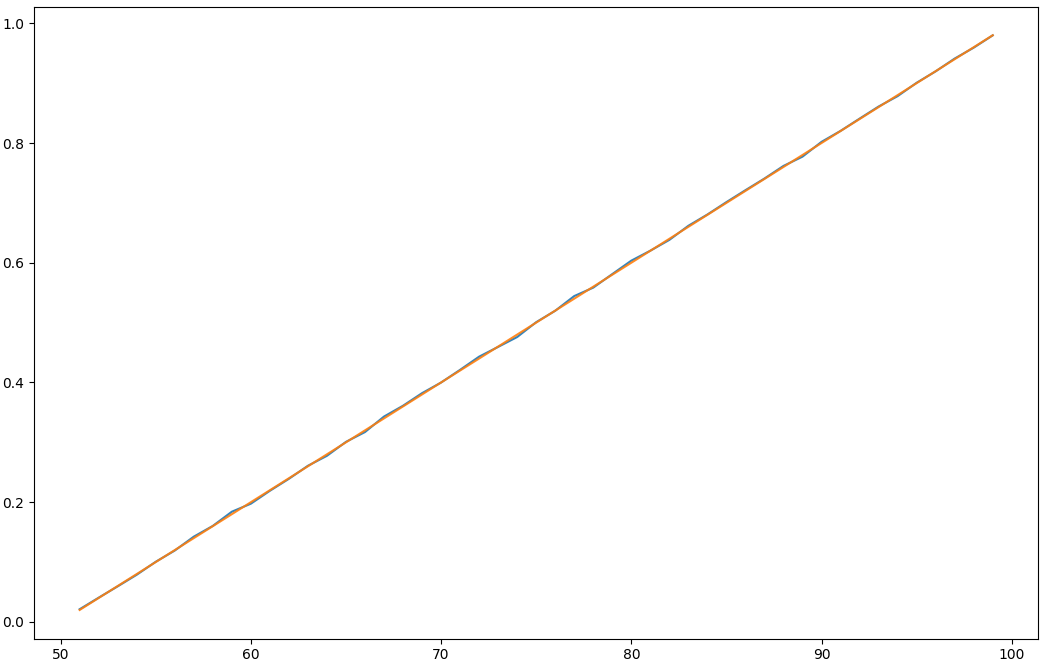
\includegraphics[scale=.55]{prob_thing_rwhw2p5.png}
    
\end{enumerate}

\newpage
\section*{Appendix}
%\lstinputlisting[language=Python]{randomwalks.py}
I did not have time to modify my code to make it faster using array operations.\\
Problem 4
\lstinputlisting[language=Python]{rw-hw2.py}
Problem 5
\lstinputlisting[language=Python]{rw-hw2-p5.py}








\end{itemize}

\end{document}


